%!TEX root = vaisagh_thesis.tex

\chapter{An Information Processing Based Approach to Modelling Perception}
\label{chapter:IBP}

% The aim of this thesis is to create an agent based fire egress simulation that models human behavior as accurately as possible.
A core component of an agent based crowd simulation is the model of movement that is used. Naturally, there has been a lot of work done on developing realistic movement models. As with any system, the effectiveness of a movement model depends on its input; in this case it is the model of perception that is used. However, this also an aspect of motion planning that is generally not given much consideration. In this chapter, we demonstrate how a more realistic model of perception can improve results produced by existing motion planning systems. This is done through a model of perception that takes into consideration the limitations of human perception.

As discussed in the previous chapters, Agent Based Simulation has recently become the preferred approach to simulating crowds because of the level of detail in which crowds can be modeled. Agent-Based Models (ABMs) consist of large-numbers of heterogeneous, autonomous entities inhabiting a spatially explicit, partially observable environment; macro level dynamics are said to emerge through the asynchronous interactions among these entities~\cite{Bonabeau:2002um,Epstein:1999vn}. Each of these individual entities will iterate through a sense-think-act cycle~\cite{IntelligentAgentsWoolridge}, where agents obtain information from their environment through {\em sensing}, make a decision through {\em thinking} and finally carry out their decision by {\em acting}. In many application areas in which ABMs have been applied, including crowd simulation, the emphasis is generally on describing thought processes accurately via rules. However, sensing is a critical aspect in the modelling process and can greatly impact both the individual and emergent properties of the system.

The terms perception and sensing are often used interchangeably in the simulation literature. For clarity in explanation, the term {\em perception} is used here to refer to the complete process of obtaining a set of (possibly filtered) \emph{percepts}~\cite{Russel:1995vi} from the environment. {\em Sensing}, on the other hand, is defined as the process of obtaining raw information from the environment; in this definition, and in this model, sensing is a part of perception.

The sense-think-act cycle is the process by which humans get information from the environment, process this information to make a decision and, finally, act based on the decision made. Rather than what a human sees, hears or smells, what is more important is what he can mentally process. In fact, the entire human perception system can simply be considered to be an information processing entity. This chapter presents a perception system based on the idea that perception is the process of gathering information from the environment. This is called the \emph{Information Based Perception}(IBP) system.

Miller's work~\cite{Miller:1956tr} on human cognition revealed two important characteristics of the human brain processes information:
\begin{inparaenum}
\item Humans constantly group together similar data into \emph{chunks} of information.
\item At any given time, a human can only process a limited amount of information.
\end{inparaenum}

For IBP, the assumption is made that this limited capacity results in humans being attracted towards certain kinds of information, e.g.\ a bright light or a celebrity; this, in turn, results in other information in the environment being unnoticed. By organizing information into chunks, humans are able to use their limited information processing capability more efficiently. This ability can manifest itself in different ways. It can be reasonably assumed that during motion planning, humans will process a group of people coming towards them as a single obstacle rather than many individuals. This grouping not only helps the person make use of his limited information processing capacity more efficiently,  it also helps him conform to social norms that instruct him that walking through a group of interacting people would be rude.


This chapter explains and illustrates the working and usefulness of an Information Based Perception system for agents. Its viability is demonstrated through the implementation of a simple moving agent and by incorporating information based processing into the agent's motion planning system. Besides being one of the major components of Agent Based Crowd Simulation, motion planning is also a process in which the effects of using a new perception system can be observed easily. The experiments towards the end of this chapter illustrate the significant effects that a modified sensing and perception system can have on an existing \emph{motion planning} algorithm. The results produced are also compared against real world experiments in an attempt to validate the model.

The remainder of this chapter is organized as follows: Section~\ref{IBP:ReviewPerception} gives some background on how humans perceive the world around them; following this, Section~\ref{IBP:MotionPlanning} presents an analyses some of the existing work in motion planning; the IBP model itself is introduced in Section~\ref{IBP:Theory};  Section~\ref{IBP:Results} presents the work done in visual, experimental and quantitative validation; finally, Section~\ref{IBP:Conclusion} concludes this chapter and gives an overview of the work that needs to be done.\footnote{This chapter was presented at the Cyberworlds 2011 Conference~\cite{Viswanathan:2011uy} and an extended version was published in the Transactions on Computational Science~\cite{Viswanathan:ut}. This chapter additionally contains some validation of the model against real world experimental data.}

\section{Limits of Human Perception}
\label{IBP:ReviewPerception}

In 1953, Hochberg and McAllister~\cite{Hochberg:1953eh} proposed the idea that humans try to group together similar information so that information can be encoded in the simplest possible format. They called this \emph{the simplicity principle}. This theory was further extended by Miller~\cite{Miller:1956tr} who proposed that, at any given time, humans can only process a limited amount of information. He explained this as the human short term working memory having a limited capacity. To enable humans to store more information in this limited storage space, humans ``chunk'' together similar information. It was originally proposed that the short term working memory could hold $7\pm 2$ chunks. Cowan~\cite{Cowan:2001wi} has argued that this limit is actually $4\pm 1$ for most humans. Thus, even though a person's 5 senses are giving him a constant stream of information about the world, limitations of human short term working memory force the person to act on the basis of only a fraction of this received information.

With regard to visual perception, some studies~\cite{Itti:2001wa,OReagan:1999wj,Triesch:2003vz} have shown that humans only pay attention to certain salient features in the objects that they see. This results in them not noticing changes in items that are not of interest to them. O'Reagan et al.~\cite{OReagan:1999wj} classified elements as either central interest or marginal interest elements and showed that the internal representation of the visual world is rather sparse and essentially contains only central interest information and not information of objects of marginal interest. The world that we perceive around is a combination of this sparse visual world along with the information in our working short term memory received from our other senses.

Based on these studies, for our model, we make the reasonable assumption that the human brain uses some mechanism to determine the significance of a particular \emph{raw percept}. And the short term working memory stores the most significant information in its limited capacity. It is important to realize that this significance determination is done for \emph{all} information received, regardless of the source. We call this significance, the \emph{amount of information}.

The idea of considering the human perception system as an information processing system is not unprecedented. Broadbent~\cite{Broadbent:1965is} extensively discussed the idea of using information theory for modelling human perception. Various studies were presented that indicate that humans have an upper bound on their capacity for holding information for perception. For a single dimension, this limit is roughly estimated to be about 5-6 percepts. For more than one dimension, the number of discernible alternatives is larger but not as large as would be expected if each dimension was completely independent.

The idea of humans being able to process only a limited amount of information is not new to computer animation either. Hill~\cite{Hill:1999ww} was one of the first to introduce the importance of cognition in sensing. Courty~\cite{Courty:2003hy} used a saliency map based approach and Kim et al.~\cite{Kim:2005ub} used cost-benefit analysis in a decision theory based approach to determining the interest points. Grillon and Thallman~\cite{Grillon:2009hf} automated this process of interest point determination. They used criteria like proximity, relative speed, relative orientation and periphery to determine the interestingness of various features.

The majority of existing perception systems, consider perception to be only visual perception. Even in more detailed crowd simulation systems like LEGION~\cite{Still:2000tp} and MASSEgress~\cite{Pan:2006vp} perception is implemented to aid movement by detecting other obstacles and goals to enable planning a path towards the goal and to provide a collision free motion. The IBP System implemented and demonstrated in this chapter is similarly limited, i.e.\ the IBP is modeled in the context of collision avoidance. The only information which the agents perceive are static obstacles, like walls, and dynamic obstacles, i.e.\ other agents or groups of agents. However, in theory, the concept of an information processing based perception system can be extended to include factors like perception of fire, smoke or other more complex \emph{cues}. Cues are certain changes in the environment that indicate that something is wrong or different from normal~\cite{Sime:1983uy} and modelling of cue perception is an important part of egress simulation. This will be discussed in more detail in Chapter~\ref{chapter:PreEvacuationBehavior}.

In the present model, the idea is not to model all the complexities of human perception and visual cognition; rather a perception model for producing more realistic movement in agent based simulation of crowds is presented. The next section gives a brief review of motion planning in existing crowd simulations.

\section{A Brief Introduction to Motion Planning Systems}
\label{IBP:MotionPlanning}

Navigation is defined as the process or activity of accurately ascertaining one's position and planning and following a route. Thus we use the term \emph{navigation} to refer to the complete process of how a person moves from one point to another. Navigation itself can be broadly divided into 3 (or 4 parts) as shown in Fig.~\ref{fig:NavigationArchitecture}. In this section, a brief overview of \emph{motion planning} is given. A more detailed description and analysis is given in Chapter~\ref{chapter:MotionPlannerComparison}. In a simulation, motion planning ensures that the simulated human avoids collisions during movement.

\begin{figure}[!tb]
\centering
\includegraphics[height=4in]{InfoBasedPerception/NavigationArchitecture}
\caption{Navigation Architecture}
\label{fig:NavigationArchitecture}
\end{figure}

There are several different approaches to motion planning. For example,  Okazaki and Matsushita~\cite{Okazaki:1993wh} used a magnetism based approach to motion with all agents having the same pole so that they repel each other and with the goal having the opposite pole. Klein and K\"oster~\cite{Klein:2009} used a similar approach of using coulombic charges instead of magnetic poles; they assigned positive charges to goals and negative charges to obstacles and agents. The most popular force based model, however, is Helbing's Social Force Model which is discussed in more detail later. Individual based motion planing was first introduced in the flocking model of Craig Reynolds~\cite{Reynolds:1987vm}. More recently, there have been several velocity-based approaches to motion planning, such as the synthetic vision based model~\cite{Ondrej:2010hv} and the Reciprocal Velocity Obstacle (RVO) Model~\cite{vandenBerg:2011ww,Guy:2010ko,vandenBerg:2008fu}. Of the many models, variants of RVO and Social Force~\cite{Helbing:1995ie} are the most popular.

Helbing's social forces model was first introduced in 1995~\cite{Helbing:1995ie}. In this model, each agent is modeled as a particle that has multiple forces acting on it. Repulsive forces help in collision avoidance and attractive forces model goal directed and grouping behavior. Over the years, this model has been extended and combined with other higher level behavior models. For example, in~\cite{Kamphuis:2004uu} more complicated group movement was modeled with an underlying social forces model for collision avoidance. In his thesis, Still~\cite{Still:2000tp} criticized the heavily mathematical approach which, according to him, is too complicated to be the natural way in which humans try to avoid crowds.

Another ABM that is increasingly becoming popular for collision avoidance is based on the idea of using the relative motion of objects to determine their time to collision. A velocity is then selected which maximizes this time. This algorithm, based on RVO was first extended for use with multi agent systems in~\cite{vandenBerg:2008cq}. Since then there have been several modifications and improvements to the system but the underlying algorithm still remained the same. CLEARPATH~\cite{Guy:2009gu} which mathematically optimized RVO was the first to introduce a change in the underlying algorithm. Guy et al.~\cite{Guy:2010ko} introduced an entirely new approach to RVO that was based on computational geometry and linear programming. This method further improved the efficiency and smoothness of the system and was called \emph{RVO2}. In another article, Guy et al.~\cite{Guy:2010uv} introduced a personal space factor and an observation delay making the algorithm more appropriate for virtual humans.

Guy et al.~\cite{Guy:2010uv} introduced an extension to RVO in the form of a higher level navigation based on the principle of least effort. While it is obvious that rational humans would prefer taking the path of least effort, as was explained in Section~\ref{IBP:ReviewPerception}, humans do not have perfect knowledge or perfect calculation. Also, it is arguable whether humans are always rational enough to choose least effort as their goal.

There are a number of existing motion planning methods that can effectively and efficiently calculate trajectories that avoid all collisions for agents, even in relatively dense environments. For robots and computer games, this might be the ideal goal: perfect, smooth and efficient motion. However, for applications like simulation of emergency evacuation the goal is obtaining realistic motion and not smooth and efficient motion. While humans thrive to be mechanically efficient, this is hardly always the case. There exist, among other things, social norms and limits to mental processing capabilities that prevent individuals from following their ideal preferred path.
% Also, humans do not necessarily use optimality (in any sense) to determine their preferred path.
We believe that a more realistic perception model like IBP, which takes into consideration human inadequacies and limitations, can help produce more naturalistic results~\cite{Klein:2009} with existing motion planning systems.

In this chapter two additions to general motion planning algorithms are proposed:
\begin{inparaenum}
\item Group sensing for motion planning which results in agents avoiding clusters of other agents when choosing their collision free path.
\item Filtering of percepts based on the amount of information provided to model limited information processing capabilities of human beings.
\end{inparaenum}

Guy et al.~\cite{Guy:2010uv} clustered very distant objects into KD-trees to reduce computational cost. While this might sound similar to the idea that is suggested in this chapter, there are two fundamental reasons why this is different from the algorithm presented here: Firstly, the present model uses multiple levels of clustering which will be explained in more detail in Section~\ref{IBP:Clustering}. Secondly, the motivation and hence design is significantly different: clustering in IBP is used as a reflection of how agents perceive their environment and not an optimization for collision avoidance.

In the following section a method that will emulate how humans perceive groups whenever possible and a system in which the agents avoid these groups rather than individuals is proposed. This has been done using the Evolving Clustering Method (ECM)~\cite{Song:2001vg} and computational geometry based RVO2~\cite{Wilkie:2009da}. But our approach can, in principle, use almost any clustering and collision avoidance algorithms.


\section{The Information Based Perception Model}
\label{IBP:Theory}

\begin{figure}[!t]
\centering
\includegraphics{InfoBasedPerception/PerceptionAndActing}
\caption[Perception and Acting]{An agent perceives and then acts}
\label{fig:AgentPerceptionAct}
\end{figure}

This section explains the Information Based Perception System. Figure~\ref{fig:AgentPerceptionAct} illustrates how motion planning works in an agent in terms of a sense-think-act cycle. An agent's perception can be described by a function $ f: Env \rightarrow p*$, where $p*$ is the set of percepts. Each percept $p$ is then processed by the agent in its decision making process, which in turn will determine an appropriate action for collision avoidance. In our case, the motion planning module is passed a set of percepts which consists of neighboring agents and static obstacles which it processes to find the most appropriate velocity for reaching the goal. Typically, this list of neighbors is a set of agents within some cone of vision or some distance away from the agent. In the proposed IBP, a modification to this traditional perception procedure is proposed such that it takes place in three phases: clustering, sensing and filtering. Figure~\ref{fig:AgentClusteredPerception} gives an overview of the process that is detailed in the following sections.


\subsection{Clustering}
\label{IBP:Clustering}
Central to our information based perception system is the definition of \emph{information units}. In traditional crowd simulation each individual agent or obstacle is considered as a percept, i.e. as an entity which should be processed by the motion planning system. The first assumption of our approach is that percepts can be both individuals and groups of other pedestrians. Whether an individual considers a group or individual is related to the {\em coherence} of the group and also the distance of the perceiving agent from the group. In order to achieve this, we perform a global clustering across the entire environment of agents. We create $n_l$ layers within the environment, each layer identifies and stores groups of a particular size, with increasing layer numbers storing groups of increasing size. The criteria which determines what actually constitutes a group is itself unknown and probably highly dependent on the individual. We make the assumption that only the proximity of the individuals to one another determine whether a collection of people is perceived as a {\em group}.

For reasons of efficiency we perform a single clustering (for each level) for all agents at every time-step, the consequence is that we are implicitly assuming all agents have the same notion of what constitutes a group. In reality this assumption may be too strong, different people may have different criteria for what they perceive as groups.

While there are various clustering techniques that could be used for grouping agents, we chose to use ECM~\cite{Song:2001vg} because:
\begin{inparaenum}
\item It does not require the number of clusters to be predefined and
\item It can restrict the maximum radius of a cluster.
\end{inparaenum}
It is also important to remember that this clustering is done dynamically at \emph{each step} and not as a one time calculation of groups.


\begin{figure}[!t]
\centering
\includegraphics{InfoBasedPerception/ClusterProcessing}
\caption[Breakdown of the Perception Process]{Perception in agents takes place through three stages: (1) Clustering is done at a global level. The dotted line indicates this separation. (2) Sensing is the process by which the Agents perceive only a subset of this. (3) Filtering further reduces the size of this list and models human visual cognition}
\label{fig:AgentClusteredPerception}
\end{figure}

First the number of clustering layers is decided. In Fig.~\ref{fig:ClusterLayer}, we illustrate information based perception using two layers. The algorithm starts by initializing a single agent as the first cluster, the maximum clustering radius for layer $i$, $r^{i}_{max}$ is fixed (Equations~\ref{firstLayerEq} and~\ref{secondLayerEq}). Each subsequent agent is then compared with every existing cluster to assess its suitability for addition to that cluster. Suitability is determined by the distance of the agent from the cluster. If the agent lies within an existing cluster, it is simply added to that cluster without updating either the radius or the cluster center. Otherwise, the cluster whose center is closest to the agent is determined. If the agent can be added to this cluster, without exceeding the maximum allowed radius for the cluster, then the agent is added to the cluster and the cluster's radius, center and velocity are updated. On the other hand, if adding the agent violates the maximum radius criteria, then a new cluster is created at the location of the agent.

Once this process is completed for layer $i$, the process is repeated for layer $i+1$ until the clusters for all the layers are determined. This process is illustrated figuratively in Fig.~\ref{fig:AgentClusteredPerception}. The clustering function for layer $i$, $cf_{i}$ allocates one and only one cluster for each agent in each later. This can be represented mathematically as shown below:
\begin{equation}
   \forall a_{k} {\in} A \mbox{ }\exists j \in  [1 , m] \quad cf_{i} : a_{k} {\rightarrow} C_{ij} \mbox{ where } 1 {\leq} m {\leq} n
\end{equation}
\begin{equation}
  \\ \forall a_{j} \in A \quad C_{0j} = a_{j}
\end{equation}
\begin{equation}
 \\r^{1}_{max} = 2 \alpha * r_{a}
  \label{firstLayerEq}
\end{equation}
\begin{equation}
  \\ \forall i \geq 2 \quad   r^{i}_{max} = 2 \alpha * r ^{i-1} _{max}
   \label{secondLayerEq}
\end{equation}

Here $r_{a}$ is the average radius of an agent\footnote{In the experiments at the end of this chapter, it is assumed that all agents have the same radius. Hence, the radius of every agent is the same as the average radius.} in $A$, which is the set of all agents; $C_{ij}$ indicates cluster $j$ in layer $i$; $m$ is the number of clusters and $n$ is the number of agents. $\alpha$ is a parameter that determines the size of clusters and the range of each region (Fig.~\ref{fig:ClusterLayer}). Through experimentation we found an $\alpha$ value of 2 to be the most suitable.

The ECM based clustering for each layer considers each agent exactly once, so the process has an asymptotic complexity of O($n^2$). At the end of each clustering, each agent belongs to a cluster. However, in the absence of nearby agents this might be a singleton cluster.

To correct certain undesirable behavior produced by ECM clustering, a modification was made to the algorithm. With large values of $r_{max}$, there is a chance that distant agents might be grouped into sparse clusters. To counter this problem, we define an \emph{inspection area} as a circle of radius $2 \alpha r_{a}$. If there are no agents within this inspection area, then the cluster is considered sparse and the cluster is removed. The sparseness check is done five times: First with the inspection area centered at the center of the cluster; and subsequently with the inspection areas centered at a distance equal to half the distance from the center of the cluster along each of the coordinate axes.

\subsection{Sensing}
\label{IBP:Sensing}

Once the agents have been clustered, the next step is to make use of these clusters for motion planning. As previously explained, existing motion planning algorithms need a list of nearby agents and obstacles to determine the most appropriate velocity. The sensing module of our proposed perception mechanism uses the set of $n_l$ layers created in the clustering module. The list of things to avoid will now consist of agents, obstacles and groups of agents. This list of nearby objects is now calculated from the multiple clustering layers as shown in Fig.~\ref{fig:ClusterLayer}.

\begin{figure*}[!t]
\centering
\includegraphics[width=\textwidth,height=3.5in]{InfoBasedPerception/AttemptedClusterLayer}
\caption[A Multi-layered Clustering Approach]{The figure illustrates how the opaque agent senses objects using 2 clustering layers. The bottom layer is the original environment and the two planes above show the two clustering layers. Clusters in layer 2 are generally bigger than in layer 1. Solid lined circles indicate the normal agents and the clustered agents. The dashed line demarcates the regions of perception. }
\label{fig:ClusterLayer}
\end{figure*}


From each cluster layer (explained in Section~\ref{IBP:Clustering}) a {\em perception region} $pr_i$ is defined for each agent. This region can be considered as a modification of the sensor range which is used in most ABM and is assumed to be a ring-shaped region.  In the first region ($pr_0$), immediately surrounding the agent performing the sensing, the agent perceives other individual agents from the clustering layer 0. This region extends to a distance $r_{pr_0} = 2\alpha *r_{a}$ from the agent's current location. For each subsequent region, the ring shaped region of sensing is from the boundary of the previous layer's region to the boundary of a circle of radius $2\alpha$ times the radius of the preceding region. So for region $pr_1$ the agent perceives groups of maximum size $r^{1}_{max}$, as long as the nearest edge of their minimum enclosing circle is within a distance $d$, such that $ r_{pr_0} < d \leq r_{pr_1}$. The result is a list of obstacles which consists of clusters of various sizes and individual agents.

\subsection{Filtering}
\label{IBP:Filtering}

As explained in Section~\ref{IBP:ReviewPerception}, a human being does not cognitively process every single object or obstacle that is within its sensing range. In other words, an agent can only process a limited amount of information and the information that is processed will be that which is deemed most interesting or important to the agent. So each object in the list obtained from perception is assigned an interestingness score of between 0 and 1 (or greater than 1 for exceptional cases discussed later). During the sensing process each agent is given an information limit $il_a$, indicating the total amount of information that can be processed by the agent. This limit is a parameter than can then change as the stress level or other characteristics of the agent changes~\cite{Ozel:2001tn}.

For now, it is assumed that interestingness of an object depends on two criteria:
\begin{inparaenum}
\item The distance of the object from the agent.
\item The angle that the object currently forms with the direction of motion of the agent.
\end{inparaenum}
A third factor indicating the innate interestingness of the object being perceived can also be used. This can be used as an aggregate to represent a lot of other properties related to interestingness. For example, an object's speed, color, action or something more subjective, i.e.\ it is of interest only to this agent because of certain properties of the agent. For e.g., for a thirsty agent, a water cooler would be interesting, whereas it is unlikely to catch the attention of someone else. A more exact definition of interestingness is not the focus of this chapter, but the general model should be able to adapt to more sophisticated definitions. However, a notion of interestingness is required to extend IBP to detect events and cues in the situation and environment.

Based on the two criteria, a score is given to each agent. A distance score of $S_{d_{immed}}>1$ is given if the distance between two agents is less than or equal to zero. This is to ensure that in high density scenarios where a collision does occur, a collision recovery mechanism is forced on the objects regardless of what angle or how interesting the object is. Too large a value would mean that too few other obstacles would be considered leading to new collisions. Through experimentation, we found a value of $S_{d_{immed}}=1.5$ produced suitable results. Beyond this, within a certain range, the distance score is fixed at $1.0$. This is considered to approximate the normal sensing range of the agent and is fixed at $7m$. Beyond this, the distance score is assumed to fall exponentially. The following equation defines this function:
\begin{equation}
  	S_d = max(min(1.0, e^{\gamma / d} - k),0.1)
\end{equation}
 $\gamma$ and $k$ are parameters which were fixed at $5.0$ and $1.11$ respectively to get a curve as in Fig.~\ref{fig:DistanceScore}.

\begin{figure}[!t]
\centering
\includegraphics[width=0.7\textwidth]{InfoBasedPerception/DistanceScore}
\caption[Distance Score]{This graph shows the variation of distance score with distance (in metres) used in experiments. A score of $S_{d_{immed}}>1$ is given if a collision has already occurred. Through experimentation this was fixed at $1.5$. The model assumes that within a certain distance agents are almost definitely perceived regardless of their distance. A distance score of 1 is assigned to objects in this range; the distance score beyond this decreases exponentially with distance.}
\label{fig:DistanceScore}
\end{figure}

An angle score of $1.0$ is given to all objects forming an angle of less than $a_{min}$ with the agent's direction. For all agents that form an angle of more than $a_{max} $ with the agent's direction,  a score of $ (1-\beta) $ is given. For our experiments a $\beta$ value of $0.9$ was used and this is illustrated in Fig.~\ref{fig:AngleScore}. For all angles in between, the angle score linearly decreases to $ (1-\beta) $ from $1$. This is assigned based on the following equation (Fig.~\ref{fig:AngleScore}). All angles are in radians:
\begin{equation}
	S_{\theta} = 1.0 - (\beta * (a - a_{min} ) / (a_{max}-a_{min}))
\end{equation}



The final score for the object is calculated as the product of the $S_{\theta}$ and $S_d$~(as long as the distance score is not $1.5$). This list of objects is then sorted on the basis of the score that is determined. Objects are then taken from the head of this list in turn and added to the final list of perceived objects as long as the cumulative score of all the perceived objects does not exceed the information limit for the agent, $il_a$. All the remaining objects are dropped from the list of objects sensed and the final list of percepts $p*$ is obtained. In case two objects have the same score, the objects that are moving towards the perceiving agent are given precedence, subsequently closer objects are given preference.

\begin{figure}[!t]
\centering
\includegraphics[width=0.7\textwidth]{InfoBasedPerception/AngleScore}
\caption[Angle Score]{This graph shows the variation of angle score with the angle(in radians) formed by the object with the agent used in experiments. For objects forming an angle of less than $70^{\circ}$ (viewing angle $140^{\circ}$, a score of 1 is given. For objects forming an angle of up to $90^{\circ}$, the score linearly decreases to $0.1$ which is the angle score for all remaining obstacles.}
\label{fig:AngleScore}
\end{figure}

This shortened neighbor list is passed as input to RVO2~\cite{Guy:2010ko} for calculating the velocity at each time step. Our hypothesis is that the 3-step perception process presented in this chapter provides an improvement in two ways: Firstly, there are fewer neighbors and hence, fewer constraints for a given sensor range. Secondly and more importantly, more natural results can be obtained as will be illustrated in Section~\ref{IBP:Results}.

\section{Model Evaluation}
\label{IBP:Results}

This section evaluates the validity of the model in three ways. First, Section~\ref{sec:model_demonstration} presents a visual and quantitative demonstration of the usefulness of the proposed model. Following this, in Section~\ref{sec:validation_against_standard_scenarios}, it is demonstrated that in standard scenarios the IBP enhanced RVO2 model produces results that are at least as good, if not better, than those obtained by using a traditional sensor range. Finally, Section~\ref{sec:experimental_validation} validates the model against real world experiments.


\subsection{Model demonstration} % (fold)
\label{sec:model_demonstration}


The ideas introduced in Section~\ref{IBP:Theory} are used as the basis for visually validating different aspects of the proposed model. For quantitative validation of the model, two measures are used: \emph{Effort Expended} and \emph{decision inconvenience Cost}. In proposing their least effort based approach to motion planning~\cite{Guy:2010uv}, Guy et al. used a measure of effort expended to demonstrate the usefulness of their model. This effort was calculated as follows:

\begin{equation}
\label{eq:energyEquation}
E = m \int \! (e_s + e_w |\vec{v}| ^2) \, \mathrm{d} t \quad \footnote{$e_{s} = 2.23 \frac{J} {Kg s}$ and $e_{w} = 1.26 \frac{Js} {Kg m^{2}}$ for an average human~\cite{Whittle:2006vsa}}
\end{equation}

In this section, the same measure of effort is used to analyze and validate the proposed IBP model. For simplicity, all agents are taken to have the same average mass of 70~kg.  However, this only measures the  mechanical effort involved. To measure the amount of effort spent in decision making, an \emph{decision inconvenience cost} measurement is introduced. The decision inconvenience cost is the number of time steps in which the agent chose a velocity other than its preferred velocity i.e., the number of times they had to avoid a collision.

Four different scenarios are considered to evaluate the overall performance. First, the effect that Group Based Perception can have on an agent moving through a crowd is demonstrated and the scenario is visually and quantitatively analyzed. Next, the effect of the multi-layered clustering on an agent moving towards a large group is similarly analyzed. Following this, the necessity of Group Based Perception (GBP) in modelling the information processing limits of human beings is shown. Finally, the importance and relevance of the information threshold is demonstrated by demonstrating the effect that it can have on an agent.

\subsubsection{Group Based Perception}
\label{GBP}

\begin{figure}[!tb]
  \centering
   \subfloat[Traditional Circular Sensor Range]{\label{Exp1_RVO}\includegraphics[width=\textwidth]{InfoBasedPerception/Exp1_RVO}}
  \\
   \subfloat[Group Based Perception]{\label{Exp1_GBP}\includegraphics[width=\textwidth]{InfoBasedPerception/Exp1_GBP}}
   \caption{Experiment 1: Group Based Perception}
  \label{Exp1}
\end{figure}


In this experiment the results of using RVO2 with a traditional simple circular sensor range against RVO2 with a Group Based Perception system is shown. The intention is to show the effect of perceiving agents as groups. The hypothesis is that by perceiving groups as obstacles the simulation will generate more natural motion. In Fig.~\ref{Exp1}, there is a single black agent moving towards the right, and a number of groups of red agents moving towards the left. The black trail shows the path that is taken by the black agent. It can be seen that in Fig.~\ref{Exp1_RVO} where GBP was not used, the agent walks through other groups. Since RVO2 enforces each agent to do half the work to avoid collision, the agents within the group individually give way through its center for the oncoming agent to pass. However, as shown in Fig~\ref{Exp1_GBP}, the GBP algorithm is capable of generating motion which avoids entire groups. The argument that this is more natural is based on the discussion in Section~\ref{IBP:ReviewPerception}; due to social norms and the human tendency to group information together people generally try to move around an entire group rather than walking directly through a group.

\begin{table}[tbp]
\caption{Quantitative analysis of Group Based Perception}
\begin{tabular}{>{\centering}p{1.2in}>{\centering}p{1in}>{\centering}p{1in}>{\centering}p{1in}>{\centering}p{1in}}
\tabularnewline
\hline\hline %inserts double horizontal lines
\multirow {2}{*}{Agent Considered} & \multicolumn{2}{c}{Effort ($ J{m}^{-1}* 10^5$)} & \multicolumn{2}{c}{Decision Inconvenience Cost}\\
 & Without GBP & With GBP & Without GBP & With GBP
 \tabularnewline
\hline
Black Agent  & 71730 & 71726 & 120 & 148 \tabularnewline
All other agents (average) & 1884 & 1880 & 14.28 & 6.56 \\
\tabularnewline
\hline
\end{tabular}
\label{tab:Exp1_QuantitativeAnalysis}
\end{table}

An analysis of the effort expended and the decision inconvenience cost gives some interesting results. Since the simulation is executed for a given number of time steps, the effort expended is normalized with the progress towards the agent's goal. This is to avoid slow or stationary agents from being considered to be more efficient despite traveling a lesser distance. On comparing the normalized effort in the two scenarios of the black agent, it is found that despite having a much longer path, the GBP enabled agent expends slightly lesser (practically the same) amount of effort than the other. This is because the non-GBP agent has to slow down to wait for the other agents to give way before it can proceed and thus progresses less towards the goal.

The decision inconvenience cost comparison gives another interesting, though not surprising, result. The decision inconvenience cost to the black agent of using Group Based Perception is higher because of the more indirect path that it has to take. However, the average decision inconvenience caused to all the other agents is significantly lesser. This is consistent with the general human reluctance to decision inconvenience others. It also gives the interesting idea that even if the same amount of mechanical effort is expended in following two different paths, the amount of decision making required for each path might be significantly different.

\subsubsection{Effects of multi layered clustering}

\begin{figure}[!t]
  \centering
   \subfloat[Using traditional sensing]{\label{Exp2_RVO}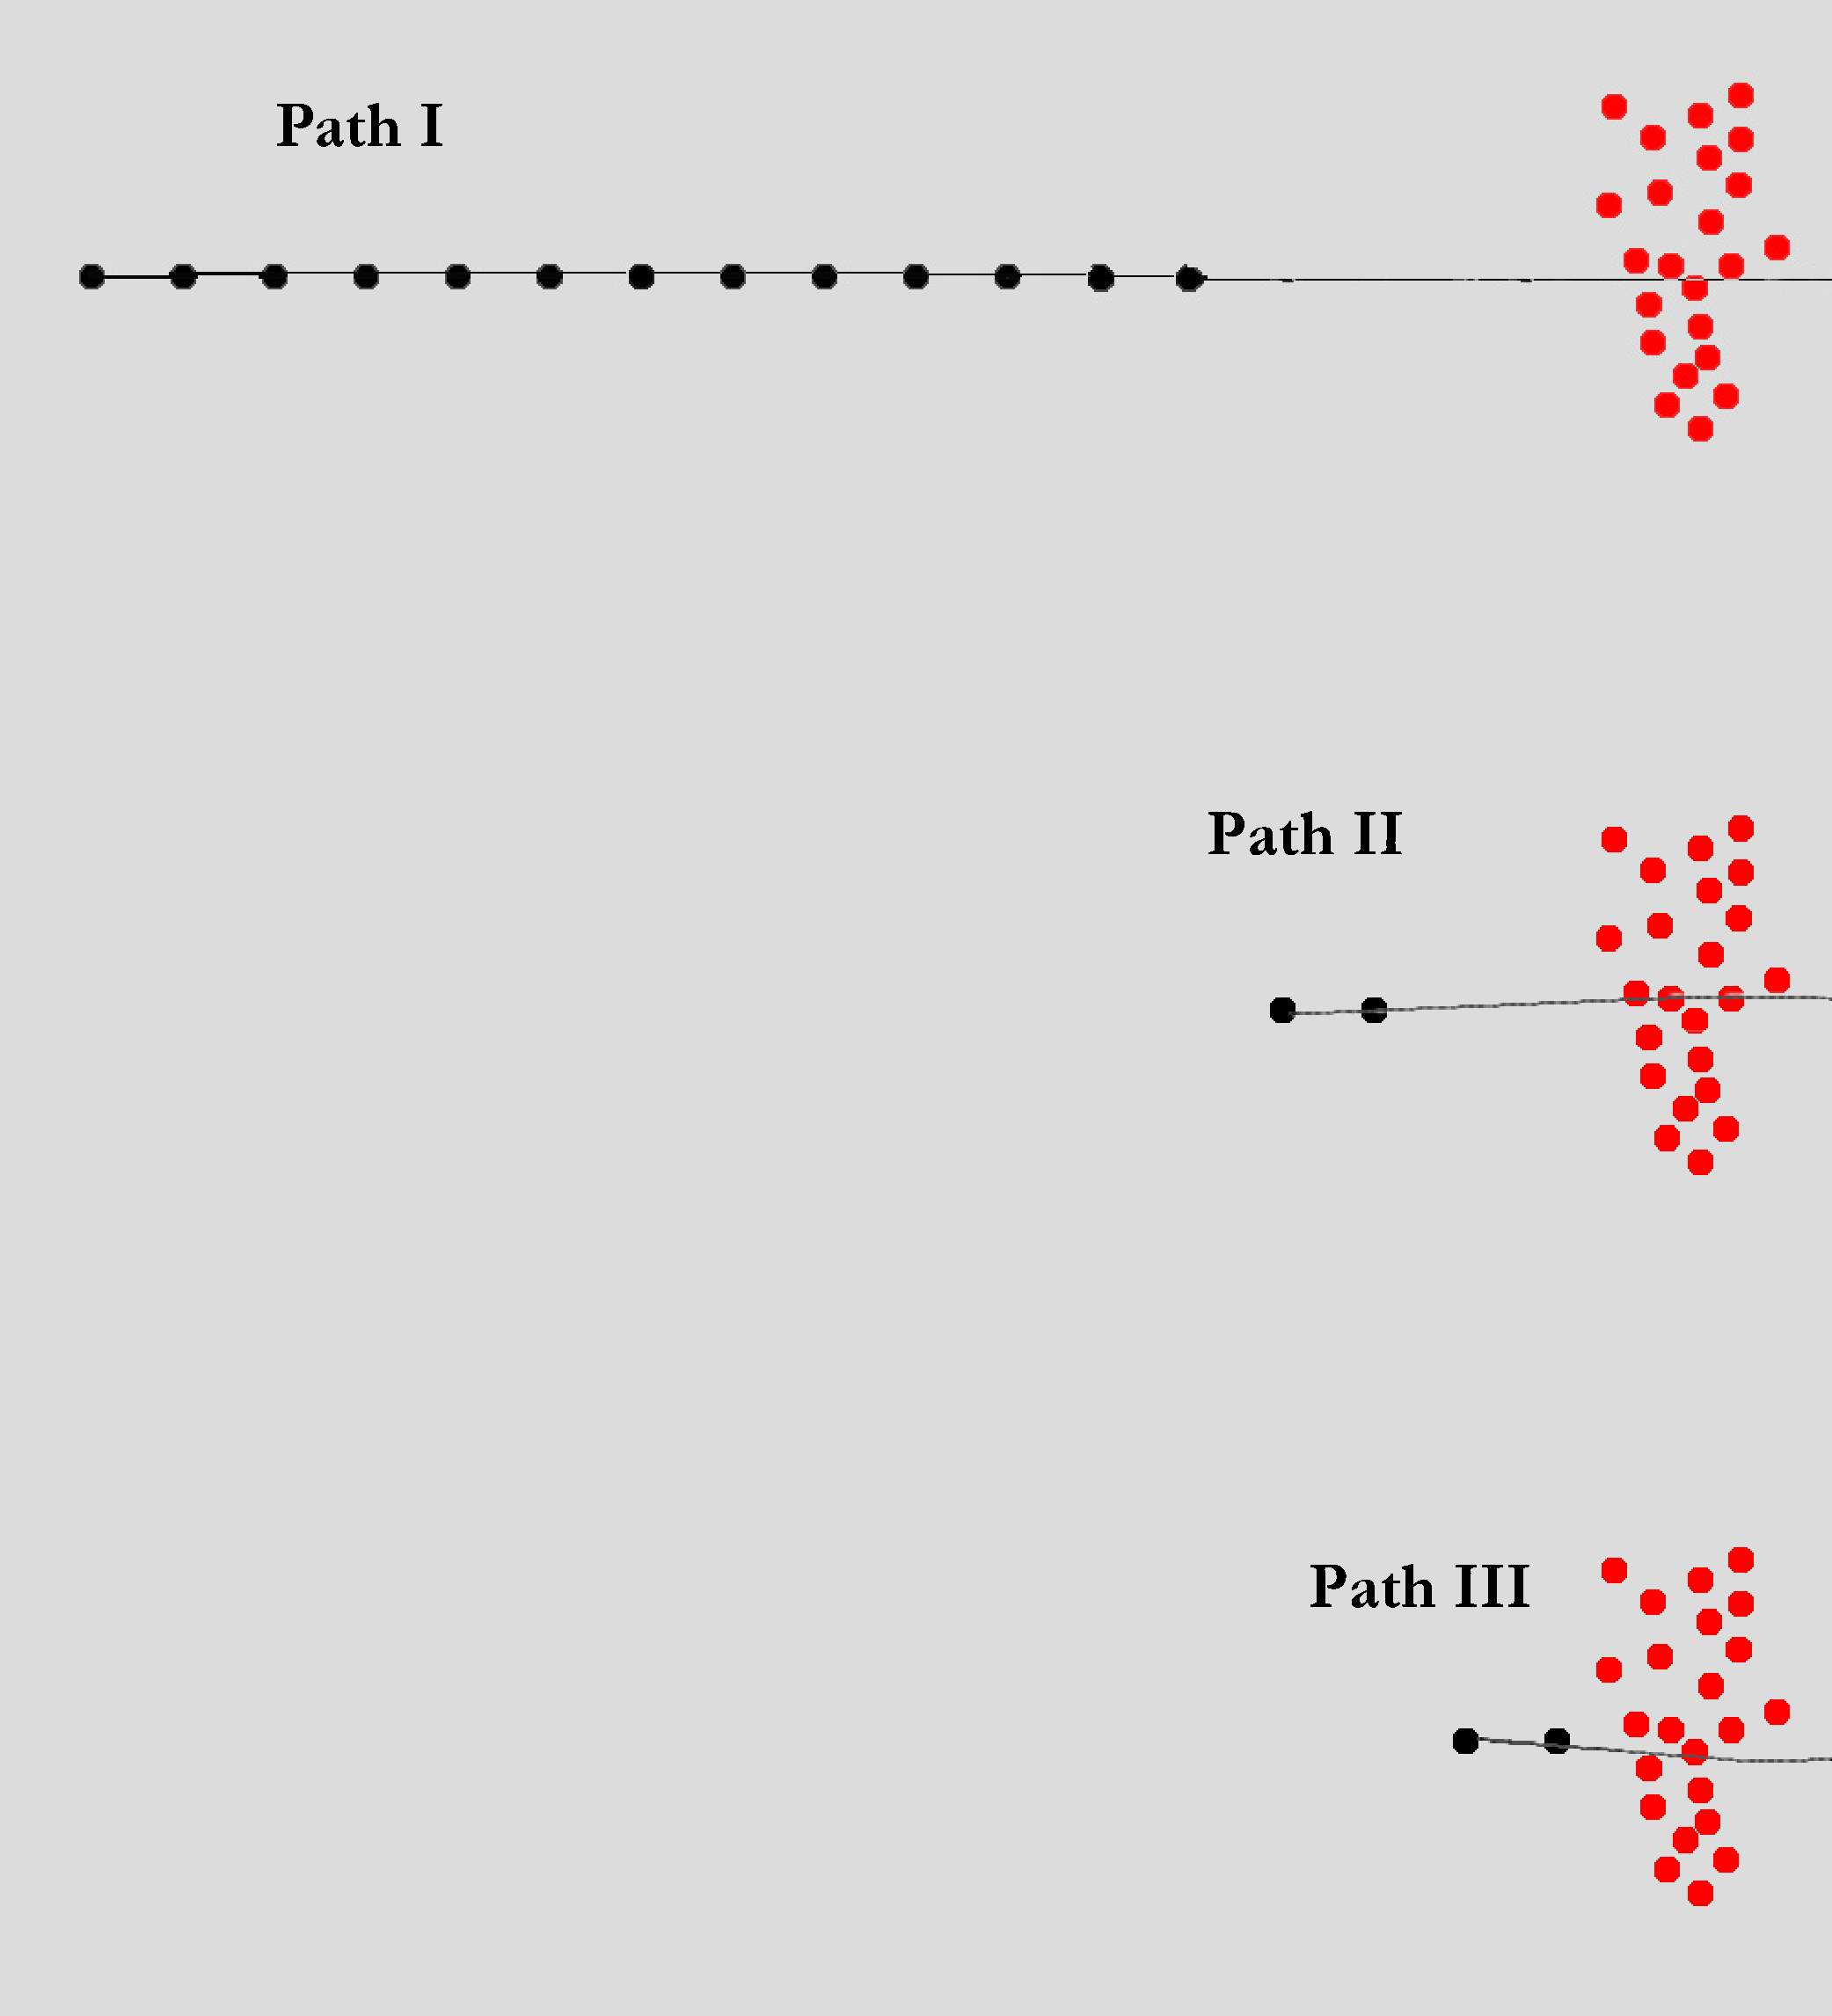
\includegraphics[width=7.5cm,height=12cm]{InfoBasedPerception/Exp2_RVO2}}
   \hspace{1pt}
  \subfloat[Using Group Based Perception]{\label{Exp2_GBP}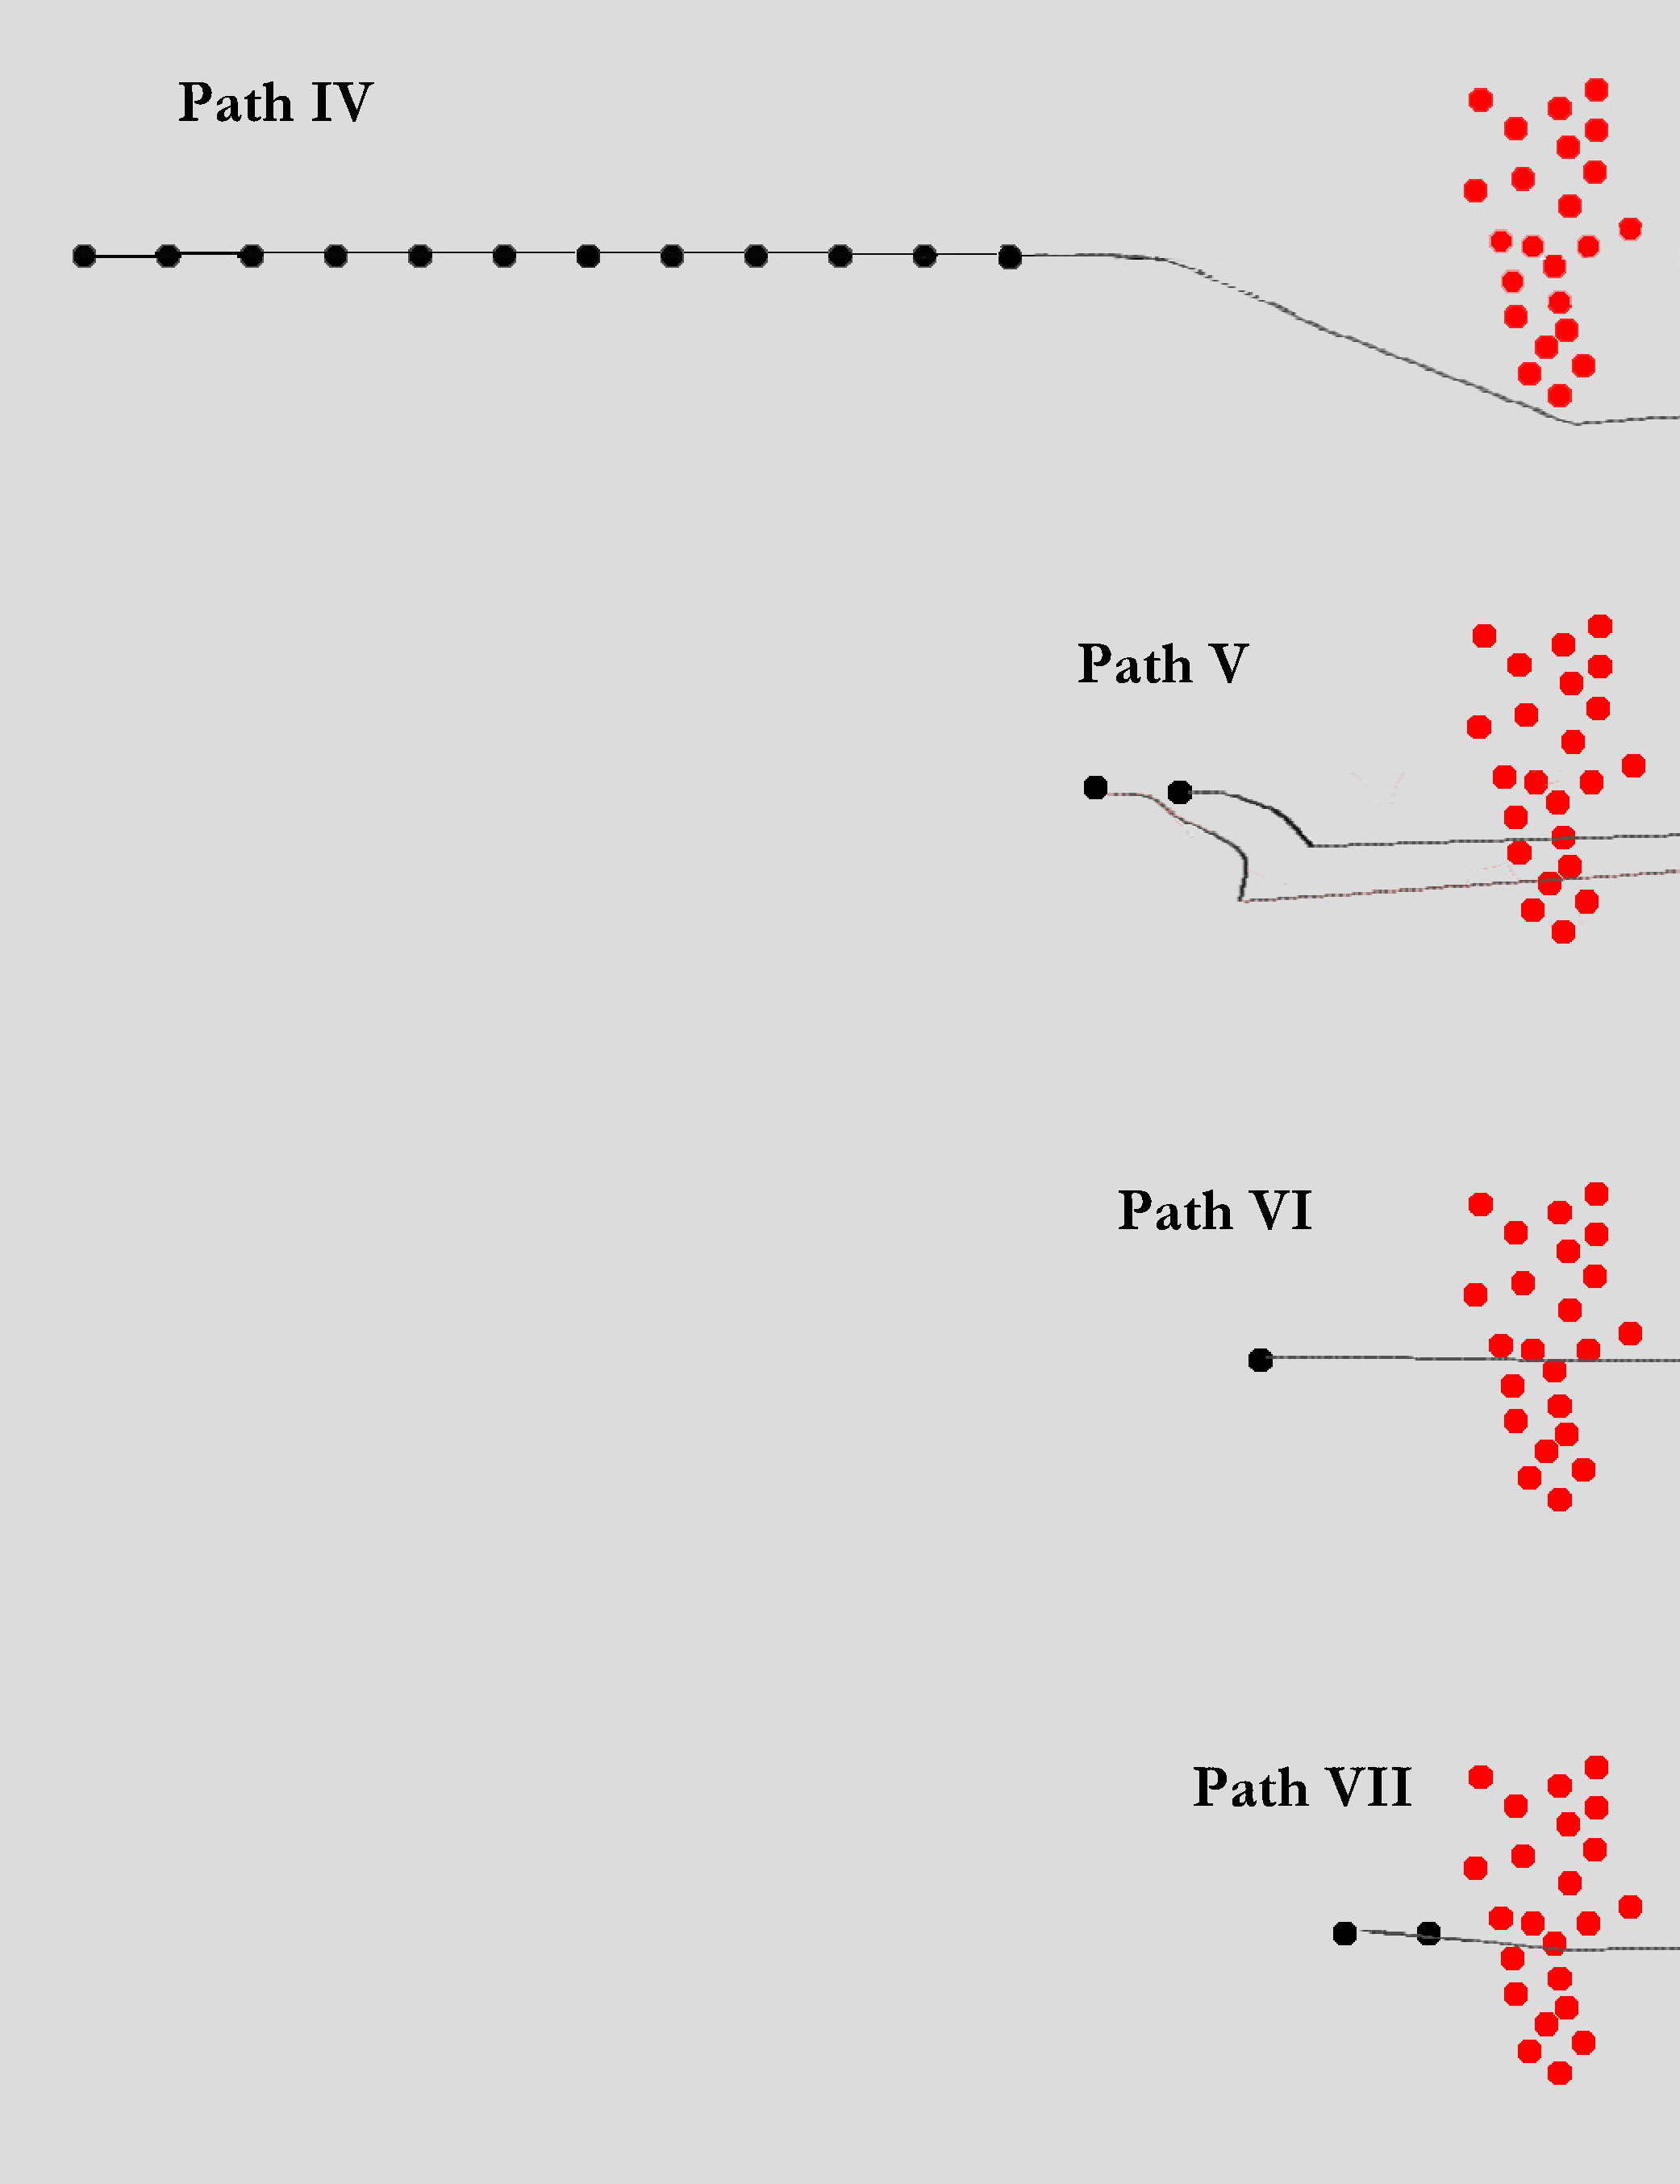
\includegraphics[width=7.5cm,height=12cm]{InfoBasedPerception/Exp2_GBP}}
  \caption{Experiment 2: Effect of multi layered clustering}
  \label{Exp2}
\end{figure}

In this experiment, the simple scenario where a single (black) agent had to get past a big group of agents to get to its goal is studied. The same experiment was performed by keeping the agent at different distances from the group. The objective of this experiment is two-fold. Firstly, it demonstrates the importance and the working of the multi-layered clustering (Section~\ref{IBP:Sensing}) used. Secondly, it demonstrates that when agents are very close to each other, where RVO2 already performs well, the Group Based Perception does not interfere with RVO2's functioning.

To recap, the multiple layers are used to describe groups of varying size at varying ranges of perception. This means agents will perceive other agents as groups or individuals depending on the distance; as an agent moves towards a group it will start to perceive the group as individual agents.

When GBP isn't used, the path followed does not change significantly with distance. The agents in the path of the black agent, give way to the agent, and the black agent just proceeds straight through the center of the large group (Path I in Fig.~\ref{Exp2_RVO}). In the last few cases (Paths II and III), the path is slightly different because the black agent does not have enough time to plan for a smooth, straight path and hence there is a slight deviation. Also, similar to the experiment in Section~\ref{GBP} it is forced to slow down in the process.

The result produced when GBP is used is more varied. Four distinctly different paths (labeled IV, V, VI and VII in Fig.~\ref{Exp2_GBP}) are produced based on how far the oncoming black agent is from the big group. At distances between 7-18m away from the center of the big cluster, the agent has enough time to perceive the group and avoid it completely (Path IV). At distances between 5-7m away, due to the size of the group, the agent gets too close to the group such that it then perceives the group as individuals. At this time (as described in Fig.~\ref{fig:ClusterLayer}) the agent performs motion planning on all the individual agents and as a consequence moves through the group, shown by path V. Path VI is obtained in a similar fashion; however, the black agent is too close to the group (4m away) to discern the effect of GBP. At distances closer than this (2-3m away), the path followed by the agent (Path VII) is exactly the same as that followed by the agent not using Group Based Perception (Path III). We argue that this type of flexibility in the perception of groups is critical to creating more natural behavior, humans will adapt what they perceive based on success or failure of their attempt to avoid larger groups.

\begin{figure}[!t]
  \centering
   \subfloat[Black Agent- Effort]{\label{Exp2_Black_Effort}\includegraphics[width=7.5cm,height=5cm]{InfoBasedPerception/Exp2_Black_Effort}}
  \hspace{1pt}
    \subfloat[Black Agent- Decision Inconvenience]{\label{Exp2_Black_decision_inconvenience}\includegraphics[width=7.5cm,height=5cm]{InfoBasedPerception/Exp2_Black_inconvenience}}
  \\
  \subfloat[Remaining Agents- Effort]{\label{Exp2_Remaining_Effort}\includegraphics[width=7.5cm,height=5cm]{InfoBasedPerception/Exp2_Remaining_Effort}}
  \hspace{1pt}
  \subfloat[Remaining Agents- Decision Inconvenience]{\label{Exp2_Remaining_decision_inconvenience}\includegraphics[width=7.5cm,height=5cm]{InfoBasedPerception/Exp2_Remaining_inconvenience}}
  \caption{Experiment 2: Quantitative Analysis}
  \label{Exp2_QuantitativeAnalysis}
\end{figure}

Figures~\ref{Exp2_Black_Effort} and \ref{Exp2_Remaining_Effort} show a comparison of the effort expended by the black agent and the average effort expended by all the remaining agents while using a traditional sensor range and GBP. As in the previous experiment (Section~\ref{GBP}) there is hardly any difference in the effort expended in both scenarios (except for a slight increase for path V). However, an interesting pattern can be observed in the decision inconvenience measurement (Figures~\ref{Exp2_Black_decision_inconvenience} and \ref{Exp2_Remaining_decision_inconvenience}). Firstly, the decision inconvenience for the rest of the group, is always lesser when GBP is used and almost the same for the black agent when path IV is followed. However, when path V or VI is followed there is a spike in the decision inconvenience curve. This can be explained by considering the fact that in both path V and VI, the black agent changes its planned path suddenly and decides to go through the group, thus not only increasing its own decision inconvenience but also the decision inconvenience caused to others in the group who have to move to give way to the agent. Finally, when path VII is followed both the effort and decision inconvenience count are exactly the same as for path III.

\subsubsection{Filtering necessitates Group Based Perception}


\begin{figure}[!t]
  \centering
  \subfloat[Initial Scenario]{\includegraphics[height=5cm]{InfoBasedPerception/Exp3_initial}}
   \\
    \subfloat[Info limit of 4, without GBP]{\label{Exp3_4_RVO}\includegraphics[width=7.5cm,height=4cm]{InfoBasedPerception/Exp3_4_RVO}}
    \hspace{1pt}
   \subfloat[Complete knowledge, without GBP]{\label{Exp3_full_RVO}\includegraphics[width=7.5cm,height=4cm]{InfoBasedPerception/Exp3_full_RVO}}
  \\
  \subfloat[Info limit of 1, with GBP]{\label{Exp3_1_GBP}\includegraphics[width=7.5cm,height=4cm]{InfoBasedPerception/Exp3_1_GBP}}
  \hspace{1pt}
  \subfloat[Info limit of 4, with GBP]{\label{Exp3_4_GBP}\includegraphics[width=7.5cm,height=4cm]{InfoBasedPerception/Exp3_4_GBP}}
  \caption{Experiment 3: The necessity of Group Based Perception}
  \label{Exp3}
\end{figure}

In Section~\ref{IBP:Theory}, the fact that humans have limited information processing capacity was explained. In this experiment, it is demonstrated that if a human being's limited information processing capability is to be modeled, it is necessary to use Group Based Perception. This is done by observing the simple scenario of an agent moving towards two groups of other agents (Fig.~\ref{Exp3}). When no information limit is imposed on the agent, and a normal circular sensor range is used, the agent, as expected, follows a nice straight path through the center of the group. However, when an information limit of $il_a = 4$ is imposed on the agent, the black agent, does not perceive all the individual agents in the group and  as a result it is forced to reconsider its path mid-route. As a result, the irregular trail shown in Fig.~\ref{Exp3_4_RVO} is obtained. However, in the same situation, when Group Based Perception is used, the agent smoothly avoids the whole group (Fig.~\ref{Exp3_4_GBP}). In fact, this smooth path is obtained for as low a limit as $il_a = 1$ (Fig.~\ref{Exp3_1_GBP}).

\subsubsection{Effect of filtering of percept information}

The final experiment (Fig.~\ref{Exp4}) demonstrates the effect of filtering, i.e.\ having limits on the information processing capabilities of the agents. The scenario consists of an agent moving towards a collection of individuals (moving towards the agent) followed by a group of agents behind the set of individuals. In the first case an information limit of $il_a = 5$ is set so that the agent is continually capable of perceiving a larger number of other agents and groups. In the second scenario a lower limit of $il_a = 3$ is used such that the agent isn't initially capable of perceiving the group behind the individuals. Figure~\ref{Exp4_5_1} shows how agents perceive the cluster that is farther away, even when there is an immediate collision to avoid. Figure~\ref{Exp4_5_2} shows that the agent manages to move around this group because it had a head start in planning - i.e.\ , it considered the group early when avoiding collisions. In the second scenario it could process a maximum of 3 or 4 percepts at any given time because of the lower information limit. Due to this, as seen in Fig.~\ref{Exp4_3_1}, the agent cannot see beyond the immediate obstacles in front and does not prepare in advance to avoid the larger group. Once the agent finally perceives this group, it is too late to move around this group as it perceives the group as individuals and then moves through the group as in Fig~\ref{Exp4_3_2}.


\begin{figure}[!tb]
  \centering
   \subfloat[Initial Scenario]{\includegraphics[height=5cm]{InfoBasedPerception/Exp4_initial}}
   \\
   \subfloat[InfoLimit 3: Step 1]{\label{Exp4_3_1}\includegraphics[width=7.5cm,height=4cm]{InfoBasedPerception/Exp4_3_1}}
  \hspace{1pt}
    \subfloat[InfoLimit 5: Step 1]{\label{Exp4_5_1}\includegraphics[width=7.5cm,height=4cm]{InfoBasedPerception/Exp4_5_1}}
  \\
  \subfloat[InfoLimit 3: Step 2]{\label{Exp4_3_2}\includegraphics[width=7.5cm,height=4cm]{InfoBasedPerception/Exp4_3_2}}
  \hspace{1pt}
  \subfloat[InfoLimit 5: Step 2]{\label{Exp4_5_2}\includegraphics[width=7.5cm,height=4cm]{InfoBasedPerception/Exp4_5_2}}
  \caption{Experiment 4: Effect of filtering of percept information}
  \label{Exp4}
\end{figure}

This experiment illustrates how small differences in the information limit can generate different forms of behavior in the agents. Interestingly, the info limit of 3 and 5 correspond to Cowan's finding~\cite{Cowan:2001wi} that all humans can cognitively process only 3-5 chunks of information at any given time. Clearly the value of the limit is critical to behavior, it is also proposed that this limit will change with personal characteristics and the emotional state of the agents. In fact this varying limit of perception may be an important factor for collisions in actual crowds, this is especially relevant in emergency egress scenarios where stress and collisions are critically important to safety planning. We plan to attempt to quantify this information limit through experimentation in future work.


In this section, we demonstrated the capabilities and the usefulness of the Information Based Perception system in Motion Planning by analyzing the effect of group based perception, multi-layered clustering and the filtering of information. In the next section, we demonstrate that RVO2 when used with IBP produces results that are at least as good as with a traditional sensor range by analyzing its performance in standard scenarios.

\subsection{Validation against standard scenarios} % (fold)
\label{sec:validation_against_standard_scenarios}

Several studies have identified standard scenarios against which motion planning systems have to be validated empirically. Hu~\cite{hunanThesis} classified these scenarios based on their main motion axes (\emph{mma}) into three main categories. Based on this categorization, he identified that validation against scenarios with 1, 2 and greater than 2 \emph{mmas} would be necessary to validate a model. In this section, we demonstrate that in these three standard scenarios, IBP enhanced RVO2 produces motion similar to traditional RVO2. For a more detailed discussion on the setup of these scenarios and the reason for this categorization, the reader is directed to Hu's thesis~\cite{hunanThesis}.
% section validation_against_standard_scenarios (end)

\subsubsection{Corridor (1 \emph{mma})} % (fold)
\label{sec:corridor}

Hu et al.~\cite{hunanThesis} identified a corridor with agents starting at either end and moving towards each other as the standard scenario in this category. Figure~\ref{fig:standard_corr} illustrates the simulation results produced by RVO2 with a traditional simple circular sensor range against RVO2 with a Group Based Perception system. An empirical observation of the simulation results does not seem to indicate much difference between the two models.


\begin{figure}[!t]
    \centering
        \subfloat[IBP - $10$ seconds]{\label{standard_corr_ibp_1}\includegraphics[width=7.5cm]{InfoBasedPerception/corr-IBP-2}}
            \hspace{1pt}
        \subfloat[RVO2 - $10$ seconds]{\label{standard_corr_rvo_1}\includegraphics[width=7.5cm]{InfoBasedPerception/corr-RVO-2}}
            \\
        \subfloat[IBP - $15$ seconds]{\label{standard_corr_ibp_2}\includegraphics[width=7.5cm]{InfoBasedPerception/corr-IBP-4}}
            \hspace{1pt}
        \subfloat[RVO2 - $15$ seconds]{\label{standard_corr_rvo_2}\includegraphics[width=7.5cm]{InfoBasedPerception/corr-RVO-4}}
                \\
        \subfloat[IBP - $17.5$ seconds]{\label{standard_corr_ibp_3}\includegraphics[width=7.5cm]{InfoBasedPerception/corr-IBP-5}}
            \hspace{1pt}
        \subfloat[RVO2 - $17.5$ seconds]{\label{standard_corr_rvo_3}\includegraphics[width=7.5cm]{InfoBasedPerception/corr-RVO-5}}
        \\
        \subfloat[IBP - $20$ seconds]{\label{standard_corr_ibp_4}\includegraphics[width=7.5cm]{InfoBasedPerception/corr-IBP-6}}
            \hspace{1pt}
        \subfloat[RVO2 - $20$ seconds]{\label{standard_corr_rvo_4}\includegraphics[width=7.5cm]{InfoBasedPerception/corr-RVO-6}}
    \caption[Corridor Experiment Screenshots]{Corridor Experiment: Scenario with 1 main motion axis. With IBP, the lane formation is slightly more asymmetric}
    \label{fig:standard_corr}
\end{figure}
% section corridor (end)

Traditionally, in this scenario, it is expected that the pedestrian agents form lanes to handle the counter flow and prevent jamming~\cite{PhysRevE.85.066128}; this is seen in both models in Figure~\ref{fig:standard_corr}. Based on more detailed studies done in~\cite{PhysRevE.85.066128}, Hu et al. suggested several qualitative measurements of the lane formation phenomenon. Firstly, they observed that lanes with a longer lifetime can more reliably reduce jams and disordered flow. As seen in the figure, both models simulated seem to produce lanes that last the length of the simulation. They also suggested that, due to the pedestrians'�� anticipation, lanes start to form early. As Figure~\ref{standard_corr_ibp_1} illustrates, with group based perception, the agents at the edges starts forming lanes even earlier than traditional RVO2 does. \cite{PhysRevE.85.066128} also stated that two or three asymmetric lanes are more realistic than a larger number of symmetric lanes. The simulations seem to indicate that when IBP
 is used, the lanes produced by the RVO2 agent become more asymmetric and arguably more realistic.

Thus, it can be seen that, in this scenario, RVO2 with IBP qualitatively produces results that are at least as good as traditional RVO2. This is further confirmed by the average effort expended calculation shown in Table~\ref{tab:energy} where both models have similar values. The effort expended was calculated as in Section~\ref{sec:model_demonstration}, using Equation~\ref{eq:energyEquation}.

\subsubsection{Intersection (2 \emph{mma})} % (fold)
\label{sec:cross}

In this category, the typical scenario identified is an intersection of two corridors with groups of pedestrians crossing each other at the intersection. Figure~\ref{fig:cross} illustrates the results of the simulation. The figure indicates that group based perception does not make much difference in this scenario. Lanes are similarly formed in both scenarios with most agents passing through smoothly. However, due to the group based perception, the efficiency and symmetry of this movement is somewhat reduced with one agent being dragged out of its preferred path by the other group because it initially tries to avoid the group. However, the calculation of the average effort per person shown in Table~\ref{tab:energy} indicates that this is not that significant a difference. Moreover, it is difficult to argue which of the two results are more accurate without experimental data.

\begin{figure}[!tp]
    \centering
        \subfloat[RVO2+IBP-200 seconds]{\label{standard_cross_ibp_1}\includegraphics[width=4.9cm]{InfoBasedPerception/cross-IBP-1}}
            \hspace{1pt}
        \subfloat[RVO2+IBP-250 seconds]{\label{standard_cross_ibp_2}\includegraphics[width=4.9cm]{InfoBasedPerception/cross-IBP-2}}
            \hspace{1pt}
        \subfloat[RVO2+IBP-300 seconds]{\label{standard_cross_ibp_3}\includegraphics[width=4.9cm]{InfoBasedPerception/cross-IBP-3}}
            \\
        \subfloat[RVO2+IBP-350 seconds]{\label{standard_cross_ibp_4}\includegraphics[width=4.9cm]{InfoBasedPerception/cross-IBP-4}}
            \hspace{1pt}
        \subfloat[RVO2+IBP-400 seconds]{\label{standard_cross_ibp_5}\includegraphics[width=4.9cm]{InfoBasedPerception/cross-IBP-5}}
            \\
        \subfloat[RVO2-200 seconds]{\label{standard_cross_rvo_1}\includegraphics[width=4.9cm]{InfoBasedPerception/cross-RVO-1}}
            \hspace{1pt}
        \subfloat[RVO2-250 seconds]{\label{standard_cross_rvo_2}\includegraphics[width=4.9cm]{InfoBasedPerception/cross-RVO-2}}
             \\
        \subfloat[RVO2-300 seconds]{\label{standard_cross_rvo_3}\includegraphics[width=4.9cm]{InfoBasedPerception/cross-RVO-3}}
             \hspace{1pt}
        \subfloat[RVO-350 seconds]{\label{standard_cross_rvo_4}\includegraphics[width=4.9cm]{InfoBasedPerception/cross-RVO-4}}
    \caption[Intersection Experiment Screenshots]{Intersection Experiment: IBP seems to marginally reduce the efficiency with which collisions are avoided in this scenario. However, this is the case only for one agent.Moreover, it is difficult to determine which result is more accurate.}
    \label{fig:cross}
\end{figure}
% section corridor (end)



\subsubsection{Circle (multiple \emph{mma})} % (fold)
\label{sec:circle}

The third and final category identified in~\cite{hunanThesis} was also the most complicated in that there are several mmas. The scenario considered to best represent this category is one with 32 agents in a circular formation. Each agent tries to exchange positions with the agent diametrically opposite to it. Collision avoidance algorithms, like RVO2, are expected to smoothly navigate this situation without a deadlock developing. For IBP to be practical, it is expected that IBP does not adversely affect the effectiveness with which RVO2 handles this difficult scenario. As shown by the trails in Figure~\ref{fig:circle} and Table~\ref{tab:energy}, this is indeed the case. Despite the trails produced being different in some ways, deadlocks do not appear and the average total effort per person is only marginally higher when IBP is used.


\begin{figure}[!t]
    \centering
        \subfloat[RVO2+IBP]{\label{circle_ibp_1}\includegraphics[scale=0.5]{InfoBasedPerception/circle32-IBP-RVO2}}
            \\
        \subfloat[RVO]{\label{circle_ibp_2}\includegraphics[scale=0.5]{InfoBasedPerception/circle32-RVO2}}
    \caption[Circle Experiment Screenshots]{Circle Experiment: IBP does not have a significant impact on the results produced by RVO2 in this scenario. Unnatural deadlocks do not develop in either scenario.}
    \label{fig:circle}
\end{figure}
% section corridor (end)


\begin{table}[!t]
\label{tab:energy}
\centering
%     \begin{adjustbox}{width=\textwidth,center}
    % \begin{adjustbox}{center}
        \begin{tabular}{p{2in}   p{2in}   p{2in} p{2in}}
                \hline
            \multicolumn{1}{c}{Model} &\multicolumn{1}{p{1.2in}}{Corridor (kJ/person)} &\multicolumn{1}{p{1.2in}}{Intersection (kJ/person)} &\multicolumn{1}{p{1.2in}}{Circle (kJ/person)}   \\
                \hline
                \hline
            \multicolumn{1}{l}{IBP+RVO2} & \multicolumn{1}{l}{152.725} & \multicolumn{1}{l}{141.183}& \multicolumn{1}{l}{115.802}
            \\%\cline{2-5}
                \hline
            \multicolumn{1}{l}{RVO2} & \multicolumn{1}{l}{152.355} & \multicolumn{1}{l}{141.193}& \multicolumn{1}{l}{111.207}
                \\%\cline{2-5}
                \hline
                \hline
        \end{tabular}
%     \end{adjustbox}
%     \vspace{ - 05 mm}
    \caption[Table summarizing effort expended for standard scenarios]{This table shows the average energy expended per agent in standard scenarios and compares the results of RVO2 with traditional sensing against RVO2 with IBP. There seem to be no significant differences between the models by this measure.}
\end{table}



In this section, we have demonstrated the working of RVO2 using IBP by comparing it against the RVO2 with a traditional sensor range in three standard scenarios: bi-directional corridor, a two-corridor intersection and a circle scenario. IBP produced results that were at least as good as a traditional sensor range in all three scenarios. In the next section, we validate the proposed model against real world data.

\subsection{Experimental validation} % (fold)
\label{sec:experimental_validation}

The experiments so far discussed in this section, have been based on quantitatively and qualitatively analyzing simulations in different scenarios. However, to better validate the model and the theory of group collision avoidance on which it is based it would be necessary to compare it against real world data. Hu et al.~\cite{HuNan2013,hunanThesis} conducted a series of controlled field experiments to study the interaction among individual participants and their movement in certain scenarios. In this section, the experimental setup used by Hu in his thesis is first reproduced. Following this, the results obtained are presented and compared against the results produced by RVO2 agents using Information Based Perception.

\subsubsection{Experiment setup} % (fold)
\label{sec:experiment_setup}

This section explains the experimental setup and measurements made by Hu et al. to study human movement in particular scenarios\footnote{This section simply summarizes the experiments conducted by Hu et al. to provide a context for the subsequent analysis and validation done. For a more detailed discussion please refer to the original paper and thesis.}. In the original paper three experiments were conducted, since IBP does not produce results different from the underlying motion planning algorithm used (RVO2 in this case) for two of the scenarios only the first experiment analyzing movement of pedestrians walking towards each other is presented and considered in this analysis.

\begin{figure}[!t]
    \begin{center}
        \includegraphics[width=\textwidth]{InfoBasedPerception/schematic_setup.pdf}
    \end{center}
    \caption[Schematic of layout of experiment area~\cite{hunanThesis}.]{A 13.5 m x 2.5 m area is demarcated for the experiments. The participants stand 10m apart and are directed to walk towards the other end at their prefered speed. (From~\cite{hunanThesis})}
    \label{fig:schematic_setup}
\end{figure}


The experiments were conducted at an outdoor passage outside the School of Computer Engineering in Nanyang Technological University. Figure~\ref{fig:schematic_setup} shows the setup of the experiment. Each experiment consisted of three participants (marked 1, 2 and 3) moving at their preferred speed in the given direction until they reached the goal point marked by the border of the demarcated area. Hu et al argue that this scenario is typical of several real life bi-directional movement scenarios. In order to shift attention from movement, the participants were given some simple algebraic calculations to do as they move.  The experimental setup is shown in Figure~\ref{fig:detailed_setup}. A video camera with adequate resolution was kept at fixed height above the experimental area using a horizontal tripod. The location of the camera and the lens was fixed to ensure maximum clarity and minimal distortion. Markers were kept on the experimental area to prevent participants from going outside the experimental area and to help in analysis of results obtained. Participants were also asked to wear white helmets so that the analysis from the video was accurate~\cite{W:2004tp}.


\begin{figure}[!tbhp]
    \begin{center}
        \includegraphics[]{InfoBasedPerception/detailed_setup.pdf}
    \end{center}
    \caption[Actual setup of Nan's experiments~\cite{hunanThesis}]{The experimental setup used by Hu et al.~\cite{hunanThesis} for their controlled field experiments.}
    \label{fig:detailed_setup}
\end{figure}

Videos of 20 experiments with 13 participants (9 male; 4 female) were finally analyzed for characteristic movement patterns and other metrics. The process shown in Figure~\ref{fig:the_video_extraction_process} was then used to extract the trajectories of each of the participants in each of the recorded videos. Briefly, the process was as follows: first the video was converted into a series of images at 20 frames per second which is an ideal frame rate to obtain a complete trajectory of the movement of participants. Once an image stack was obtained the image was scaled, rotated and transformed using the markers to remove distortions and bring it to metric scale. Following this, the next two steps quantize the image and remove noise such that, at the end of the process, each image only has black and white colors with the former depicting the background and the latter the participants. Lastly, an existing software is used for tracking each participant (white particle) in the quantized images. Fig.~\ref{fig:VideoExtractionExample} gives an example of the whole process.

\begin{figure}[!tb]
    \begin{center}
        \includegraphics[scale=0.75]{InfoBasedPerception/DataExtractionProcess.pdf}
    \end{center}
    \caption{The data extraction process.}
    \label{fig:the_video_extraction_process}
\end{figure}

\begin{figure}[!htb]
    \centering
   		\subfloat[Step 1]{\includegraphics[width=7.5cm,height=4cm]{InfoBasedPerception/extract_1}}
  		\hspace{1pt}
    	\subfloat[Step 2]{\includegraphics[width=7.5cm,height=4cm]{InfoBasedPerception/extract_2}}
  		\\
  		\subfloat[Step 3]{\includegraphics[width=7.5cm,height=4cm]{InfoBasedPerception/extract_3}}
  		\hspace{1pt}
  		\subfloat[Step 4]{\includegraphics[width=7.5cm,height=4cm]{InfoBasedPerception/extract_4}}
  		\\
  		\subfloat[Step 5]{\includegraphics[width=7.5cm,height=4cm]{InfoBasedPerception/extract_5}}
  		\hspace{1pt}
  		\subfloat[Step 6]{\includegraphics[width=7.5cm,height=4cm]{InfoBasedPerception/extract_6}}
  	\caption{An example of the video extraction process}
    \label{fig:VideoExtractionExample}
\end{figure}





\subsubsection{Quantitative measurements of experimental data} % (fold)
\label{sec:metrics_used}

\begin{figure}[!hb]
    \begin{center}
        \includegraphics[width=\textwidth]{InfoBasedPerception/CategoriesPicture}
    \end{center}
    \caption{The trajectories of participants can be grouped into 3 categories}
    \label{fig:categoriesOfMotion}
\end{figure}

The data extraction process outlined in Section~\ref{sec:experiment_setup} produces for each participant in each experiment a trajectory. Trajectories that were similar were grouped together and normalized to find an average trajectory for each group. It was observed that these trajectories could be grouped into three main groups shown in Figure~\ref{fig:categoriesOfMotion}.  The quantitative measurements that are explained next are all calculated on the average trajectory for each of these groups.

The different measurements used by Hu et al. are very neatly summarized in Figure~\ref{fig:OverviewOfMetrics}. These metrics are:

\begin{figure}[!htb]
    \begin{center}
        \includegraphics[width=\textwidth]{InfoBasedPerception/metricsUsedHuNan}
    \end{center}
    \caption{Metrics proposed by Hu et al. for quantitative validation of models~\cite{hunanThesis}.}
    \label{fig:OverviewOfMetrics}
\end{figure}

\begin{itemize}
    \item Trajectory length of participant $i$ ($L_i$).
    % \item Distance deviated from the horizontal direction line (along the x axis) of participant $i$ as a function of time $t$ ($dd^t_i$). The horizontal direction line is also the shortest trajectory for the participant towards his goal.
    \item Maximum deviation of participant $i$ ($D_i$). This is the maximum value of $dd^t_i$ for a participant over the course of the complete trajectory.
    % \item  The local curvature of participant $i$ as a function of time ($lc^t_i$). The local curvature of a participant at a given time is the tangent of the angle formed by the instantaneous velocity of the participant to the velocity along the horizontal direction line.
    % \item The difference of local curvatures between participants $i$ and $j$ as a function of a time $t$ ($\Delta lc^t_{ij}$).
    \item The speed of the participant as function of time $t$ ($s^t_i$).
    \item The distance between agents $i$ and $j$ as a function of time $t$ ($d^t_{ij}$).
\end{itemize}

% section metrics_used (end)


\subsubsection{Results and comparison} % (fold)
\label{sec:comparison_of_ibp}

This section presents the simulation results produced using IBP when compared against the experimental data. The experimental setup was replicated by initializing the agents as shown in Fig.~\ref{fig:experiment_simulation_setup}. Of the four metrics proposed, the maximum deviation and inter-agent distance against time seemed to differentiate best between the models. Hence, in this section, we use these metrics for evaluating IBP. Appendix~\ref{cha:speed_experiment_comparison} discusses briefly the results of the other two metrics.

\begin{figure}[!b]
    \begin{center}
        \includegraphics[width=\textwidth]{InfoBasedPerception/expSimulationSetup}
    \end{center}
    \caption[Layout of experiment in simulation]{The initial configuration of the simulation based on the experimental setup in real world experiments.}
    \label{fig:experiment_simulation_setup}
\end{figure}


% The metrics in Section~\ref{sec:metrics_used} can be broadly grouped into two kinds: temporal measures and non-temporal ones.

Table~\ref{tab:RealWorldDistanceDeviation} shows the maximum deviation values for the real world data. It can be broadly seen that in $95\%$ of the cases, Participant 2 avoided Participant 1 and 3 through either side. It can also be seen that the major deviation effort was taken by single agent ($\approx 0.87m$) rather than the group of two agents ($\approx 0.2 -0.3m$). Table~\ref{tab:IBPDistanceDeviation} compares the distance deviation calculation for the simulation results against the real world data. Due to the symmetry of the behavior of agents 1 and 3 in category 1 and 2 of the real world experiments, we do not loose much information by averaging category 1 and 2 to obtain the values in the second column of Table~\ref{tab:IBPDistanceDeviation} which represents 95\% of the real world data. The remaining columns in the same table show the results produced by traditional RVO2, Social Force and RVO2 with IBP.  As can be seen, RVO2 with IBP produces the dynamics most similar to the real world experiments. This is more clearly illustrated in Figure~\ref{fig:nonTemporalIllustration}.


\begin{table}[!t]

\centering
%     \begin{adjustbox}{width=\textwidth,center}
    % \begin{adjustbox}{center}
        \begin{tabular}{p{0.75in}   p{0.75in} p{0.75in} p{0.75in}}
            \hline
            \multicolumn{4}{c}{Maximum Deviation Calculation from Experiments}  \\
            \hline
            \multicolumn{1}{c}{} &\multicolumn{1}{c}{Category 1 (\textbf{55\%})} &\multicolumn{1}{c}{Category 2 (40\%)}  &\multicolumn{1}{c}{Category 3 (5\%)} \\
            \hline
            \hline
            \multicolumn{1}{l}{Agent 1} & \multicolumn{1}{l}{0.0785} & \multicolumn{1}{l}{0.320723} & \multicolumn{1}{l}{0.241166}
            \\%\cline{2-5}
            \multicolumn{1}{l}{Agent 2} & \multicolumn{1}{l}{\textbf{0.8720}}& \multicolumn{1}{l}{\textbf{0.868398}}& \multicolumn{1}{l}{0.320865}
            \\%\cline{2-5}
            \multicolumn{1}{l}{Agent 3} & \multicolumn{1}{l}{0.2656}& \multicolumn{1}{l}{0.18667}& \multicolumn{1}{l}{\textbf{0.657496}}
                                    \\
            \hline
            \hline
        \end{tabular}
%     \end{adjustbox}
%     \vspace{ - 05 mm}
    \caption[Real world maximum deviation~\cite{hunanThesis}]{This table summarizes the maximum deviation according to experiments conducted by Hu~\cite{hunanThesis}. Category 1 refers to the movement of Agent 2 to the left of the group, category 2 to the movement of Agent 2 to the right of the group and category 3 to the movement of agent 2 through the middle of the oncoming group.}
    \label{tab:RealWorldDistanceDeviation}
\end{table}

\begin{table}[!b]
\label{tab:SimulationDistanceDeviation}
\centering
%     \begin{adjustbox}{width=\textwidth,center}
    % \begin{adjustbox}{center}
        \begin{tabular}{ p{0.75in}   p{0.75in} p{0.75in} p{0.75in} p{0.75in}}
            \hline
             \multicolumn{1}{c}{} & \multicolumn{1}{c}{Experiment (95\%)} & \multicolumn{1}{c}{IBP-RVO2} & \multicolumn{1}{c}{RVO2} & \multicolumn{1}{c}{Social Force}    \\
            \hline
            \hline
             \multicolumn{1}{l}{Agent 1} & \multicolumn{1}{l}{0.199} & \multicolumn{1}{l}{0.0} & \multicolumn{1}{l}{0.043} & \multicolumn{1}{l}{0.372}
            \\%\cline{2-5}
            \multicolumn{1}{l}{Agent 2}  & \multicolumn{1}{l}{\textbf{0.870}} & \multicolumn{1}{l}{\textbf{0.855}} & \multicolumn{1}{l}{\textbf{0.003}} & \multicolumn{1}{l}{\textbf{0.0}}
            \\%\cline{2-5}
            \multicolumn{1}{l}{Agent 3}  & \multicolumn{1}{l}{0.226} & \multicolumn{1}{l}{0} & \multicolumn{1}{l}{0.038} & \multicolumn{1}{l}{0.372}\\
            \hline
            \hline
        \end{tabular}
%     \end{adjustbox}
%     \vspace{ - 05 mm}
    \caption[Maximum deviation measurements from simulations]{This table shows the trajectory length obtained for the simulation of the experimental scenario in~\cite{hunanThesis}. The first column lists the average of category 1 and 2 which together comprised 95\% of the real world experiment data of~\cite{hunanThesis}. The same pattern of agent 2 having larger value than the other two is obtained only when IBP is used.}
    \label{tab:IBPDistanceDeviation}
\end{table}

\begin{figure}[!t]
    \begin{center}
        \includegraphics[width=0.75\textwidth]{InfoBasedPerception/maxDevIllustration}
    \end{center}
    \caption{Graphical illustration of the  absolute difference in maximum deviations that can be seen in Table~\ref{tab:energy}.}
\end{figure}

Figure~\ref{fig:DistanceIBPPlot} illustrates the inter-agent distance as a function of time for the experimental data, RVO2, Social Force and RVO2 with IBP. As in the real world experiments of Hu it can be seen that agents 1 and 3 maintain a relatively constant value. It can also be seen that, at its closest point, as in the experiment, agent 2 becomes closer to one of agent 1 and 3 than they are to each other. This is closer to the experimental data than the results produced by RVO2 and Social Force using a normal sensor range as shown in Fig.~\ref{fig:DistanceIBPPlot-RVO2} and Fig.~\ref{fig:DistanceIBPPlot-SF}.

\begin{figure}[!tb]
  \centering
  \subfloat[Experiment- Category 1 (55\%)~\cite{hunanThesis}]{\includegraphics[width=0.48 \textwidth]{InfoBasedPerception/interAgentDistanceCat1}}
  \hspace{1pt}
  \subfloat[Experiment- Category 2 (40\%)~\cite{hunanThesis}]{\includegraphics[width=0.48 \textwidth]{InfoBasedPerception/interAgentDistanceCat2}}\\
   \subfloat[IBP-RVO2]{\label{fig:DistanceIBPPlot-IBP}\includegraphics[width=0.6\textwidth]{InfoBasedPerception/DistancePlot-RVO2-IBP}}
\\
   \subfloat[RVO2]{\label{fig:DistanceIBPPlot-RVO2}\includegraphics[width=0.6\textwidth]{InfoBasedPerception/DistancePlot-RVO2}}
\\
    \subfloat[Social Force]{\label{fig:DistanceIBPPlot-SF}\includegraphics[width=0.6\textwidth]{InfoBasedPerception/DistancePlot-SocialForce}}
  \caption[Inter agent distances over time.]{Plot of inter agent distances over time for various models and the experimental data.}
  \label{fig:DistanceIBPPlot}
\end{figure}

Thus, this section has demonstrated how Information Based Perception helps RVO2 produce results that are  similar to those obtained by Hu et al. in their controlled experiments.


% section experimental_validation (end)

\section{Summary and Future Work}
\label{IBP:Conclusion}

We began this chapter with an argument that traditional spatial distance based perception systems limited the ability of existing motion planning systems to produce realistic motion.
An Information Based Perception model for agents which is based on perceived information rather than spatial distance was introduced based on existing theories of human cognition. Through simulations and comparison against real world experiments it was argued that this is a more appropriate model of human perception for crowd and egress simulation as it helped produce more realistic group avoidance behavior. The idea that humans have limited perception capacity such that they only process certain obstacles more relevant to collision avoidance was incorporated and its usefulness demonstrated. The real world experiments conducted by Hu et al. were introduced and comparison of simulation results against experimental results showed that Information Based Perception can help models like RVO2 replicate the results produced by the experiments.



The IBP model can be extended so that during filtering it can recognize cues that contain event and environment information as well. This can be passed as input to the Event Identification system which is described in more detailed in Chapter~\ref{chapter:PreEvacuationBehavior}. Also, one aspect of the model that has not been explored much is the quantification of information limits and appropriate definitions of interest; real world experiments could be conducted to attempt to quantify these parameters. The third criteria which was mentioned in Section~\ref{IBP:Filtering}, i.e.\ the inherent interestingness of perceived objects, could also be the subject of these real world experiments.

In emergency situations, according to Ozel~\cite{Ozel:2001tn}, humans start perceiving cues in the environment differently. The idea of modelling different cues and their effect on the agent's information processing capabilities as suggested by Kuligowski~\cite{Kuligowski:2009un} is an idea that will be discussed in more detail in Chapter~\ref{chapter:PreEvacuationBehavior}. As mentioned by Hill~\cite{Hill:1999ww} there is also a reciprocal effect of cognition on perception where agents would turn towards objects of more interest. These could also be incorporated into a later version of the IBP model. In the next chapter, a model for how perceived cues can be used for identifying events and modelling pre-evacuation behavior is presented.

